
%% bare_conf.tex
%% V1.4a
%% 2014/09/17
%% by Michael Shell
%% See:
%% http://www.michaelshell.org/
%% for current contact information.
%%
%% This is a skeleton file demonstrating the use of IEEEtran.cls
%% (requires IEEEtran.cls version 1.8a or later) with an IEEE
%% conference paper.
%%
%% Support sites:
%% http://www.michaelshell.org/tex/ieeetran/
%% http://www.ctan.org/tex-archive/macros/latex/contrib/IEEEtran/
%% and
%% http://www.ieee.org/

%%*************************************************************************
%% Legal Notice:
%% This code is offered as-is without any warranty either expressed or
%% implied; without even the implied warranty of MERCHANTABILITY or
%% FITNESS FOR A PARTICULAR PURPOSE! 
%% User assumes all risk.
%% In no event shall IEEE or any contributor to this code be liable for
%% any damages or losses, including, but not limited to, incidental,
%% consequential, or any other damages, resulting from the use or misuse
%% of any information contained here.
%%
%% All comments are the opinions of their respective authors and are not
%% necessarily endorsed by the IEEE.
%%
%% This work is distributed under the LaTeX Project Public License (LPPL)
%% ( http://www.latex-project.org/ ) version 1.3, and may be freely used,
%% distributed and modified. A copy of the LPPL, version 1.3, is included
%% in the base LaTeX documentation of all distributions of LaTeX released
%% 2003/12/01 or later.
%% Retain all contribution notices and credits.
%% ** Modified files should be clearly indicated as such, including  **
%% ** renaming them and changing author support contact information. **
%%
%% File list of work: IEEEtran.cls, IEEEtran_HOWTO.pdf, bare_adv.tex,
%%                    bare_conf.tex, bare_jrnl.tex, bare_conf_compsoc.tex,
%%                    bare_jrnl_compsoc.tex, bare_jrnl_transmag.tex
%%*************************************************************************


% *** Authors should verify (and, if needed, correct) their LaTeX system  ***
% *** with the testflow diagnostic prior to trusting their LaTeX platform ***
% *** with production work. IEEE's font choices and paper sizes can       ***
% *** trigger bugs that do not appear when using other class files.       ***                          ***
% The testflow support page is at:
% http://www.michaelshell.org/tex/testflow/



\documentclass[conference]{IEEEtran}
% Some Computer Society conferences also require the compsoc mode option,
% but others use the standard conference format.
%
% If IEEEtran.cls has not been installed into the LaTeX system files,
% manually specify the path to it like:
% \documentclass[conference]{../sty/IEEEtran}





% Some very useful LaTeX packages include:
% (uncomment the ones you want to load)


% *** MISC UTILITY PACKAGES ***
%
%\usepackage{ifpdf}
% Heiko Oberdiek's ifpdf.sty is very useful if you need conditional
% compilation based on whether the output is pdf or dvi.
% usage:
% \ifpdf
%   % pdf code
% \else
%   % dvi code
% \fi
% The latest version of ifpdf.sty can be obtained from:
% http://www.ctan.org/tex-archive/macros/latex/contrib/oberdiek/
% Also, note that IEEEtran.cls V1.7 and later provides a builtin
% \ifCLASSINFOpdf conditional that works the same way.
% When switching from latex to pdflatex and vice-versa, the compiler may
% have to be run twice to clear warning/error messages.






% *** CITATION PACKAGES ***
%
%\usepackage{cite}
% cite.sty was written by Donald Arseneau
% V1.6 and later of IEEEtran pre-defines the format of the cite.sty package
% \cite{} output to follow that of IEEE. Loading the cite package will
% result in citation numbers being automatically sorted and properly
% "compressed/ranged". e.g., [1], [9], [2], [7], [5], [6] without using
% cite.sty will become [1], [2], [5]--[7], [9] using cite.sty. cite.sty's
% \cite will automatically add leading space, if needed. Use cite.sty's
% noadjust option (cite.sty V3.8 and later) if you want to turn this off
% such as if a citation ever needs to be enclosed in parenthesis.
% cite.sty is already installed on most LaTeX systems. Be sure and use
% version 5.0 (2009-03-20) and later if using hyperref.sty.
% The latest version can be obtained at:
% http://www.ctan.org/tex-archive/macros/latex/contrib/cite/
% The documentation is contained in the cite.sty file itself.






% *** GRAPHICS RELATED PACKAGES ***
%
\ifCLASSINFOpdf
  % \usepackage[pdftex]{graphicx}
  % declare the path(s) where your graphic files are
  % \graphicspath{{../pdf/}{../jpeg/}}
  % and their extensions so you won't have to specify these with
  % every instance of \includegraphics
  % \DeclareGraphicsExtensions{.pdf,.jpeg,.png}
\else
  % or other class option (dvipsone, dvipdf, if not using dvips). graphicx
  % will default to the driver specified in the system graphics.cfg if no
  % driver is specified.
  % \usepackage[dvips]{graphicx}
  % declare the path(s) where your graphic files are
  % \graphicspath{{../eps/}}
  % and their extensions so you won't have to specify these with
  % every instance of \includegraphics
  % \DeclareGraphicsExtensions{.eps}
\fi
% graphicx was written by David Carlisle and Sebastian Rahtz. It is
% required if you want graphics, photos, etc. graphicx.sty is already
% installed on most LaTeX systems. The latest version and documentation
% can be obtained at: 
% http://www.ctan.org/tex-archive/macros/latex/required/graphics/
% Another good source of documentation is "Using Imported Graphics in
% LaTeX2e" by Keith Reckdahl which can be found at:
% http://www.ctan.org/tex-archive/info/epslatex/
%
% latex, and pdflatex in dvi mode, support graphics in encapsulated
% postscript (.eps) format. pdflatex in pdf mode supports graphics
% in .pdf, .jpeg, .png and .mps (metapost) formats. Users should ensure
% that all non-photo figures use a vector format (.eps, .pdf, .mps) and
% not a bitmapped formats (.jpeg, .png). IEEE frowns on bitmapped formats
% which can result in "jaggedy"/blurry rendering of lines and letters as
% well as large increases in file sizes.
%
% You can find documentation about the pdfTeX application at:
% http://www.tug.org/applications/pdftex





% *** MATH PACKAGES ***
%
%\usepackage[cmex10]{amsmath}
% A popular package from the American Mathematical Society that provides
% many useful and powerful commands for dealing with mathematics. If using
% it, be sure to load this package with the cmex10 option to ensure that
% only type 1 fonts will utilized at all point sizes. Without this option,
% it is possible that some math symbols, particularly those within
% footnotes, will be rendered in bitmap form which will result in a
% document that can not be IEEE Xplore compliant!
%
% Also, note that the amsmath package sets \interdisplaylinepenalty to 10000
% thus preventing page breaks from occurring within multiline equations. Use:
%\interdisplaylinepenalty=2500
% after loading amsmath to restore such page breaks as IEEEtran.cls normally
% does. amsmath.sty is already installed on most LaTeX systems. The latest
% version and documentation can be obtained at:
% http://www.ctan.org/tex-archive/macros/latex/required/amslatex/math/





% *** SPECIALIZED LIST PACKAGES ***
%
%\usepackage{algorithmic}
% algorithmic.sty was written by Peter Williams and Rogerio Brito.
% This package provides an algorithmic environment fo describing algorithms.
% You can use the algorithmic environment in-text or within a figure
% environment to provide for a floating algorithm. Do NOT use the algorithm
% floating environment provided by algorithm.sty (by the same authors) or
% algorithm2e.sty (by Christophe Fiorio) as IEEE does not use dedicated
% algorithm float types and packages that provide these will not provide
% correct IEEE style captions. The latest version and documentation of
% algorithmic.sty can be obtained at:
% http://www.ctan.org/tex-archive/macros/latex/contrib/algorithms/
% There is also a support site at:
% http://algorithms.berlios.de/index.html
% Also of interest may be the (relatively newer and more customizable)
% algorithmicx.sty package by Szasz Janos:
% http://www.ctan.org/tex-archive/macros/latex/contrib/algorithmicx/




% *** ALIGNMENT PACKAGES ***
%
%\usepackage{array}
% Frank Mittelbach's and David Carlisle's array.sty patches and improves
% the standard LaTeX2e array and tabular environments to provide better
% appearance and additional user controls. As the default LaTeX2e table
% generation code is lacking to the point of almost being broken with
% respect to the quality of the end results, all users are strongly
% advised to use an enhanced (at the very least that provided by array.sty)
% set of table tools. array.sty is already installed on most systems. The
% latest version and documentation can be obtained at:
% http://www.ctan.org/tex-archive/macros/latex/required/tools/


% IEEEtran contains the IEEEeqnarray family of commands that can be used to
% generate multiline equations as well as matrices, tables, etc., of high
% quality.




% *** SUBFIGURE PACKAGES ***
%\ifCLASSOPTIONcompsoc
%  \usepackage[caption=false,font=normalsize,labelfont=sf,textfont=sf]{subfig}
%\else
%  \usepackage[caption=false,font=footnotesize]{subfig}
%\fi
% subfig.sty, written by Steven Douglas Cochran, is the modern replacement
% for subfigure.sty, the latter of which is no longer maintained and is
% incompatible with some LaTeX packages including fixltx2e. However,
% subfig.sty requires and automatically loads Axel Sommerfeldt's caption.sty
% which will override IEEEtran.cls' handling of captions and this will result
% in non-IEEE style figure/table captions. To prevent this problem, be sure
% and invoke subfig.sty's "caption=false" package option (available since
% subfig.sty version 1.3, 2005/06/28) as this is will preserve IEEEtran.cls
% handling of captions.
% Note that the Computer Society format requires a larger sans serif font
% than the serif footnote size font used in traditional IEEE formatting
% and thus the need to invoke different subfig.sty package options depending
% on whether compsoc mode has been enabled.
%
% The latest version and documentation of subfig.sty can be obtained at:
% http://www.ctan.org/tex-archive/macros/latex/contrib/subfig/




% *** FLOAT PACKAGES ***
%
%\usepackage{fixltx2e}
% fixltx2e, the successor to the earlier fix2col.sty, was written by
% Frank Mittelbach and David Carlisle. This package corrects a few problems
% in the LaTeX2e kernel, the most notable of which is that in current
% LaTeX2e releases, the ordering of single and double column floats is not
% guaranteed to be preserved. Thus, an unpatched LaTeX2e can allow a
% single column figure to be placed prior to an earlier double column
% figure. The latest version and documentation can be found at:
% http://www.ctan.org/tex-archive/macros/latex/base/


%\usepackage{stfloats}
% stfloats.sty was written by Sigitas Tolusis. This package gives LaTeX2e
% the ability to do double column floats at the bottom of the page as well
% as the top. (e.g., "\begin{figure*}[!b]" is not normally possible in
% LaTeX2e). It also provides a command:
%\fnbelowfloat
% to enable the placement of footnotes below bottom floats (the standard
% LaTeX2e kernel puts them above bottom floats). This is an invasive package
% which rewrites many portions of the LaTeX2e float routines. It may not work
% with other packages that modify the LaTeX2e float routines. The latest
% version and documentation can be obtained at:
% http://www.ctan.org/tex-archive/macros/latex/contrib/sttools/
% Do not use the stfloats baselinefloat ability as IEEE does not allow
% \baselineskip to stretch. Authors submitting work to the IEEE should note
% that IEEE rarely uses double column equations and that authors should try
% to avoid such use. Do not be tempted to use the cuted.sty or midfloat.sty
% packages (also by Sigitas Tolusis) as IEEE does not format its papers in
% such ways.
% Do not attempt to use stfloats with fixltx2e as they are incompatible.
% Instead, use Morten Hogholm'a dblfloatfix which combines the features
% of both fixltx2e and stfloats:
%
% \usepackage{dblfloatfix}
% The latest version can be found at:
% http://www.ctan.org/tex-archive/macros/latex/contrib/dblfloatfix/




% *** PDF, URL AND HYPERLINK PACKAGES ***
%
%\usepackage{url}
% url.sty was written by Donald Arseneau. It provides better support for
% handling and breaking URLs. url.sty is already installed on most LaTeX
% systems. The latest version and documentation can be obtained at:
% http://www.ctan.org/tex-archive/macros/latex/contrib/url/
% Basically, \url{my_url_here}.




% *** Do not adjust lengths that control margins, column widths, etc. ***
% *** Do not use packages that alter fonts (such as pslatex).         ***
% There should be no need to do such things with IEEEtran.cls V1.6 and later.
% (Unless specifically asked to do so by the journal or conference you plan
% to submit to, of course. )

% package für unsere umlaute
\usepackage[utf8]{inputenc}
\usepackage[ngerman]{babel}

% correct bad hyphenation here
\hyphenation{op-tical net-works semi-conduc-tor}


\begin{document}
%
% paper title
% Linebreaks \\ can be used within to get better formatting as desired.
% Do not put math or special symbols in the title.
\title{
Dokumentation der Entwicklung des Spiels\\
No Beer is oooch No Option (NBNO)
}

% author names and affiliations
% use a multiple column layout for up to three different
% affiliations
\author{\IEEEauthorblockN{Tom Oberhauser}
\IEEEauthorblockA{Beuth Hochschule für Technik Berlin\\
Medieninformatik Master\\
Software Engineering\\
Matrikelnummer: 859851\\}
\and
\IEEEauthorblockN{Robin Mehlitz}
\IEEEauthorblockA{Beuth Hochschule für Technik Berlin\\
Medieninformatik Master\\
Software Engineering\\
Matrikelnummer: 857946\\}}

% make the title area
\maketitle

% As a general rule, do not put math, special symbols or citations
% in the abstract
\begin{abstract}
Als Semesterprojekt wird das 2D Top-Down Spiel NBNO entwickelt.
Ziel des Spielers ist es, sein Bier nicht vor Ablauf der Levelzeit leer werden zu lassen.
Zur Levelerzeugung wird eine domänenspezifische Sprache entwickelt. Mit Hilfe dieser Sprache ist es auch ohne Programmierkenntnisse möglich, neue Level zu erzeugen.
\end{abstract}


% For peer review papers, you can put extra information on the cover
% page as needed:
% \ifCLASSOPTIONpeerreview
% \begin{center} \bfseries EDICS Category: 3-BBND \end{center}
% \fi
%
% For peerreview papers, this IEEEtran command inserts a page break and
% creates the second title. It will be ignored for other modes.
\IEEEpeerreviewmaketitle



\section{Wollen wir ein datum einbinden}
\hfill mds
 
\hfill September 17, 2014


\section{Einleitung}

Diese Dokumentation gibt einen Überblick über das Semesterprojekt im Modul Software-Engineering des Masterstudienganges Medieninformatik.
Ziel des Projekts ist es, eine anwendungsspezifische Sprache (domain-specific language oder auch DSL) zu entwickeln und anhand dieser, Code einer höheren Programmiersprache zu generieren.
Der generierte Code soll hierbei eine zu implementierende Anwendung komplettieren und somit der Umgang mit anwendungsspezifischen Sprachen sowie der Codegenerierung praxisnah geübt und gefestigt werden.

Die Anforderung wird anhand eines Spiels und eines Levelgenerators umgesetzt.
Der Levelgenerator übernimmt hierbei die Verarbeitung der anwendungsspezifischen Sprache.

\subsection{Spielidee}

Es soll ein 2D Spiel in Top-Down Perspektive entwickelt werden.
Das Spielziel ist es, ein sich ständig leerendes Bier rechtzeitig durch den Besuch eines \textit{Spätis}\footnote{Späti ist eine, in Berlin gebräuchliche, Abkürzung für Spätverkaufsstelle. Spätis verkaufen, mitunter die ganze Nacht über, unter anderem Bier und sind somit die ``Tankstelle'' der trinkenden Nachtschwärmer.}
wieder aufzufüllen und bis zum Ende einer vorher definierten Zeit das Bier nicht leer werden zu lassen.
Dazu bewegt der Spieler sich in einer blockbasierten Welt.
Diese enthält sowohl Spätis zum nachfüllen des Bieres, als auch Gegner welche den Füllstand des Bieres oder die Geschwindigkeit des Spielers reduzieren können.
Gegner besitzen eine gewisse Intelligenz und können den Spieler verfolgen sobald sie ihn gesehen haben.
Abbildung \ref{fig:einleitung:screenshot} zeigt eine typische Szene des Spiels.
Die Statusbalken am unteren Bildrand geben Auskunft über den aktuellen Füllstand des Bieres (links), sowie die verbleibende Zeit (rechts) welche der Spieler überbrücken muss um das Level erfolgreich abzuschließen.

\begin{figure}[]
\centering
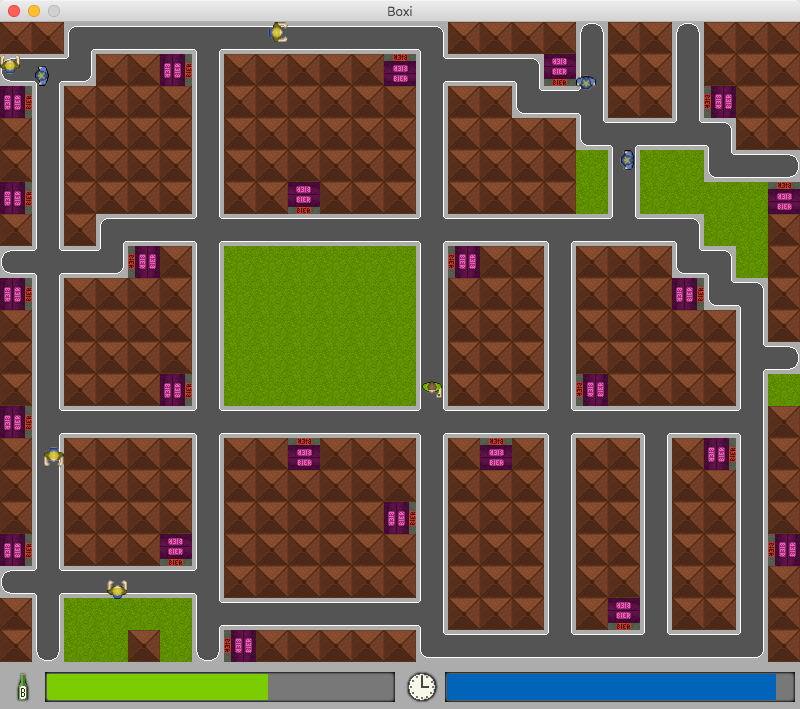
\includegraphics[width=3in]{img/02_screenshot.png}
\caption{Screenshot des Spiels}
\label{fig:einleitung:screenshot}
\end{figure}


\subsection{Zweck der Codegenerierung}

Das Spiel beinhaltet mehrere Level.
Ein Level beinhaltet beispielsweise Informationen über die Anordnung der Blöcke auf der Karte oder die Lauf- und Trinkgeschwindigkeit des Spielers.
Dazu wurde eine anwendungsspezifische Sprache und ein Codegenerator entwickelt, auf welchen in Abschnitt \ref{sec:levelerzeugung} näher eingegangen wird.
\section{Aufbau der Infrastruktur}

Das Spiel sowie auch der Levelgenerator werden mittels der Programmiersprache Java 8 entwickelt. 
Als Entwicklungsumgebung dient das IntelliJ IDEA System.\todo{Sätze verbinden oder System umformulieren.}
Beide Programme werden jeweils in einem eigenen IntelliJ Projekt implementiert.
Dadurch ist eine strikte Unabhängigkeit zwischen dem Levelgenerator und dem Spiel gewährleistet.

Um die Teamarbeit effizient zu gestalten, wird das Versionierungswerkzeug Git\footnote{https://git-scm.com} eingesetzt.
Es ermöglicht die Zusammenarbeit über die Plattform GitHub\footnote{https://github.com}, auf der verschiedene nützliche Features angeboten werden.
Sehr häufige Verwendung in diesem Projekt findet die Erzeugung und Zusammenführung von Pull Requests.
Nachdem ein Entwickler ein Feature entwickelt oder einen Fehler behoben hat, wird so ein Pull Request erstellt.
Ein weiteres Teammitglied überprüft diese Codeänderung und merged sie, bei positivem Ergebnis, auf die Master Branch.

Eine weitere wichtige GitHub Funktion besteht im Erstellen von sogenannte Issues.
Dies sind Repository interne Forumseinträge, die bestimmte Projektbezogene Themen behandeln sollen.
Es können durch Labels Rubriken festgelegt werden, wie zum Beispiel ``Bug`` oder ``Question``.
So erhält das Projekt eine Struktur und Entscheidungen bzw. Hinweise die für das gesamte Team wichtig sind, werden an zentraler Stelle veröffentlicht und zur Diskussion freigegeben.

Für das Bauen und die Verwaltung von Abhängigkeiten zu Bibliotheken und Frameworks wird im Spieleprojekt das Tool Maven verwendet.
Im Generator Projekt dagegen besteht keine Notwendigkeit für ein solches Tool, weshalb hier Maven nicht eingesetzt wird.

\section{Technologien}

Das Spiel sowie der Levelgenerator benutzen Bibliotheken und Frameworks. Dabei spielt die Slick2d Abhängigkeit im Spiele Projekt und die Antl Benutzung im Generator die größte Rolle. Diese beiden Frameworks werden im Folgenden näher erläutert.
\subsection{Slick2D}

Zur Entwicklung des Spiels wird die \textit{Slick2D}\footnote{http://slick.ninjacave.com} Bibliothek verwendet.
Slick2D basiert auf der \textit{Lightweight Java Game Library (LWJGL)}\footnote{https://www.lwjgl.org}.
LWJGL ist eine sehr umfangreiche Bibliothek, welche viele für unseren Anwendungsfall benötigte Funktionalitäten bereitstellt.
Dazu gehören die hardwarenahe Erzeugung grafischer Bildschirmausgabe via OpenGL, sowie die Verarbeitung von Tastatureingaben.
Slick2D bildet eine Abstraktionsschicht über der LWJGL, speziell für den Anwendungsfall der 2D Spieleentwicklung.
Dies ermöglicht eine effiziente Spieleentwicklung.
\subsection{Antlr}

Der Levelgenerator soll aus einer textbasierten Datei eine Java Klasse erstellen. Dafür wird ein Parser, sowie ein Lexer benötigt. Um diese nicht selbst zu schreiben, wird das Werkzeug \textit{Antlr (v4)} verwendet.

Antlr ist ein Quellcodegenerator, der Parser und Lexer in einer vom Nutzer ausgewählten Programmiersprache erstellt. Dabei ist Java die Standardeinstellung. Die Dateien werden anhand einer vom Entwickler vorgegebenen Grammatik generiert. \footnote{www.antlr.org/about.html} 

Dabei ist wichtig zu verstehen, was ein Lexer und was ein Parser ist und tut. 

Ein Lexer vollzieht die lexikalische Analyse. Das bedeutet, er unterteilt den eingegebenen Text in Einheiten, sogenannte Tokens. Dies können zum Beispiel Schlüsselwörter, Zahlen oder auch Zeichenketten sein. Aufgrund dieser Einteilung kann eine zur Prüfung gegebene Datei, vollständig in Tokens zerlegt werden. 
\footnote{http://www2.math.uni-wuppertal.de/$\sim$axel/skripte/compiler/c1\_10\_1.html} 

Der Parser hingegen erstellt aus der gegebenen Datei und den erzeugten Tokens eine Struktur, die im Fall von Antlr, als Syntaxbaum generiert wird. So kann jede beliebige Datei mit Hilfe dieses Syntaxbaums, bezüglich der korrekte Struktur überprüft werden. \footnote{http://www.itwissen.info/definition/lexikon/Parser-parser.html}

Die Kombination aus Lexer und Parser ermittelt die syntaktische Korrektheit des gegebenen Textes. Sollte ein Fehler auftreten, kann aufgrund der vergebenen Tokens die exakte Zeile und Spalte in der gegebenen Datei bestimmt werden. Ist die Datei vollständig in Tokens zerlegbar und stimmt die Struktur mit den Parserregeln überein, gilt die Datei als fehlerfrei und kann benutzt werden.

Um die Regeln für den Lexer und Parser festzulegen, schreibt der Entwickler eine, auf der \textit{Erweiterten Backus-Naur-Form (EBNF)} basierende, Grammatik und generiert mittels Antlr hieraus die Lexer- und Parserklassen.

Durch Antlr werden in diesem Vorgang ebenfalls Listener erstellt, die benutzt werden können, um an bestimmten Stellen beim Parsen der Datei Zugriff auf die aktuelle Struktur und Daten zu erhalten. So kann der Programmierer semantische Prüfungen der Daten durchführen und entsprechend auf korrekte oder fehlerhafte Eingaben reagieren.

Um mit Antlr Code generieren zu können, kann in IntelliJ IDEA das Antlr Plugin installiert werden. Durch Ausführen des Plugins auf der Grammatik wird der gewünschte Java Code erstellt.

Weitere Einstellungen sind über die Konfiguration des Plugins möglich. Hier wird beispielsweise festgelegt, wohin die Lexer- und Parserdateien generiert werden sollen oder in welcher Programmiersprache diese Dateien erstellt werden. 
Sind die Lexer und Parser in das Sourcecodeverzeichnis eingebunden, so können sie in einem Java Programm aufgerufen und ausgeführt werden.



\subsection{Pixelart?}
\section{Aufbau der Spielarchitektur}
\label{sec:architektur}

\subsection{Überblick}
\label{sub:architektur:ueberblick}

Slick2D stellt Techniken zur Umsetzung eines zustandsbasierten Spieles zur Verfügung.
In Abbildung \ref{fig:spielarchitektur:states} werden die Zustände des Spiels und ihre Reihenfolge gezeigt.

Ein Spiel startet im \texttt{MainMenuState}.
Hier kann der Spieler das Spiel entweder direkt beenden oder in den \textit{LevelMenuState} wechseln.
Der \texttt{LevelMenuState} bietet eine Auswahl aller zur Verfügung stehenden Levels an, welche dann im \texttt{PlayingState} gespielt werden können.
Während des Spiels kann das Spiel durch Wechsel in den \texttt{PauseMenuState} pausiert werden.
Nach erfolgreichem oder nicht erfolgreichem Abschluss eines Levels bietet der \texttt{GameFinishState} die Möglichkeit das Level zu wechseln, das Level erneut zu spielen oder das Spiel zu beenden.

\begin{figure}[]
\centering
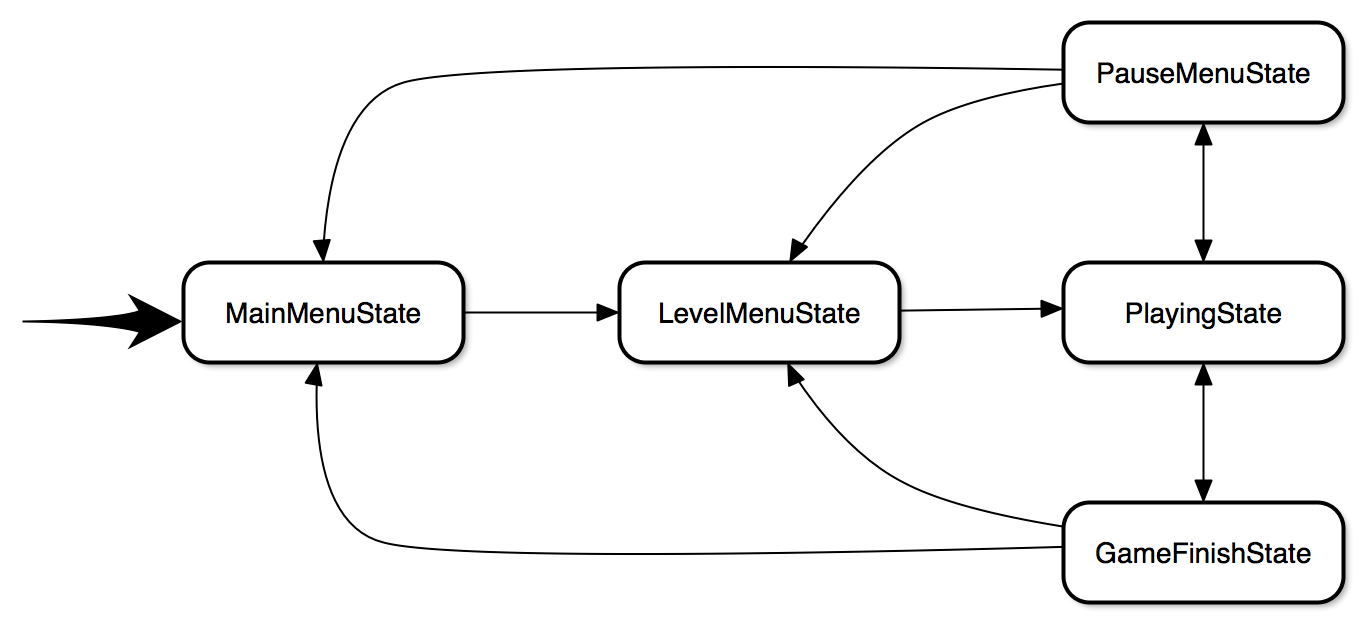
\includegraphics[width=3in]{img/05_states.png}
\caption{Übersicht der Zustände des Spiels}
\label{fig:spielarchitektur:states}
\end{figure}

Im FMC-Diagramm in Abbildung \ref{fig:spielarchitektur:fmc} wird die Bedeutung des \texttt{PlayingState} sowie der Aufbau eines Levels deutlich.
Der \texttt{PlayingState} empfängt die Eingaben des Spielers und reicht diese an den \texttt{LevelController} weiter.
Der \texttt{LevelController} kontrolliert und steuert die Bestandteile eines Levels.

\begin{figure}[]
\centering
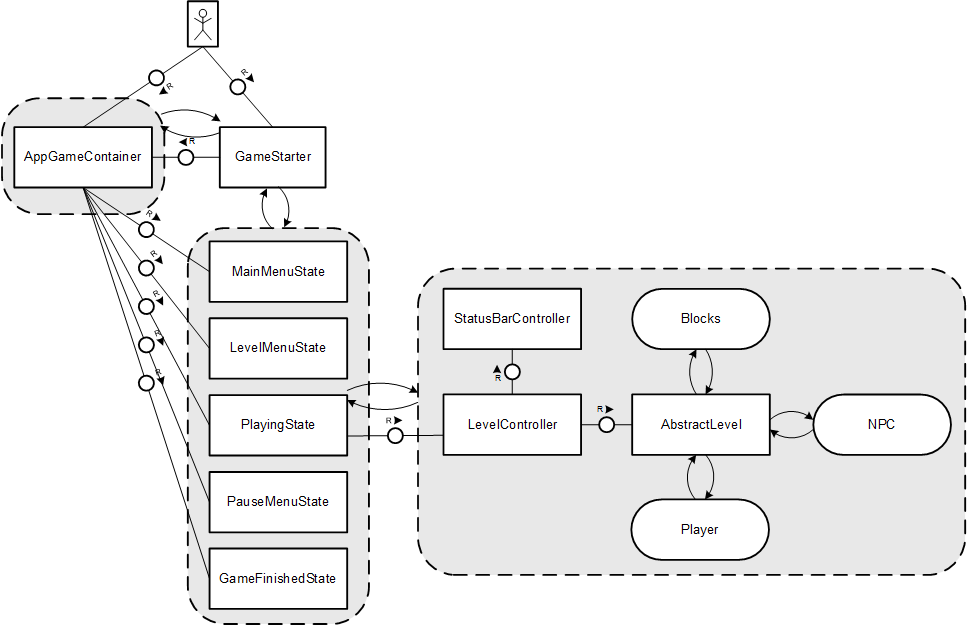
\includegraphics[width=3in]{img/05_fmc.png}
\caption{FMC Diagramm des Spiels}
\label{fig:spielarchitektur:fmc}
\end{figure}

\subsection{Level}
\label{sub:architektur:level}

Jedes Level erbt von \texttt{AbstractLevel}.
In Abbildung \ref{fig:spielarchitektur:abstractlevel} wird der Aufbau eines Levels deutlich.
Ein Level besteht aus einer Menge an \texttt{NPC}-Objekten (non-player character), welche die Gegner repräsentieren.
Außerdem beinhaltet es ein \texttt{Player}-Objekt sowie die Menge der Blöcke(\texttt{Block}), also der Karte des Levels.
Eine Übersicht über alle verwendbaren Spielobjekte wird in Abbildung \ref{fig:spielarchitektur:model} gegeben.
Level sind komplexe Datentypen und verstehen sich als Komposition der, in Abbildung \ref{fig:spielarchitektur:model} gezeigten, spielspezifischen \texttt{GameObject} Datentypen.
Zur Vermeidung von Redundanz und zur klaren Trennung zwischen Modell und Controller wird die Steuerung der Elemente eines Levels durch den \texttt{LevelController} übernommen.
Durch diese Trennung eignen sich Implementierungen von \texttt{AbstractLevel} sehr gut zur Erzeugung durch eine anwendungsspezifische Sprache.

\begin{figure}[]
\centering
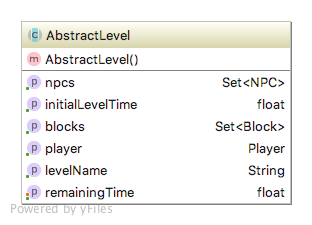
\includegraphics[width=2in]{img/05_abstractlevel_uml.png}
\caption{UML Darstellung der Klasse AbstractLevel}
\label{fig:spielarchitektur:abstractlevel}
\end{figure}

\begin{figure}[]
\centering
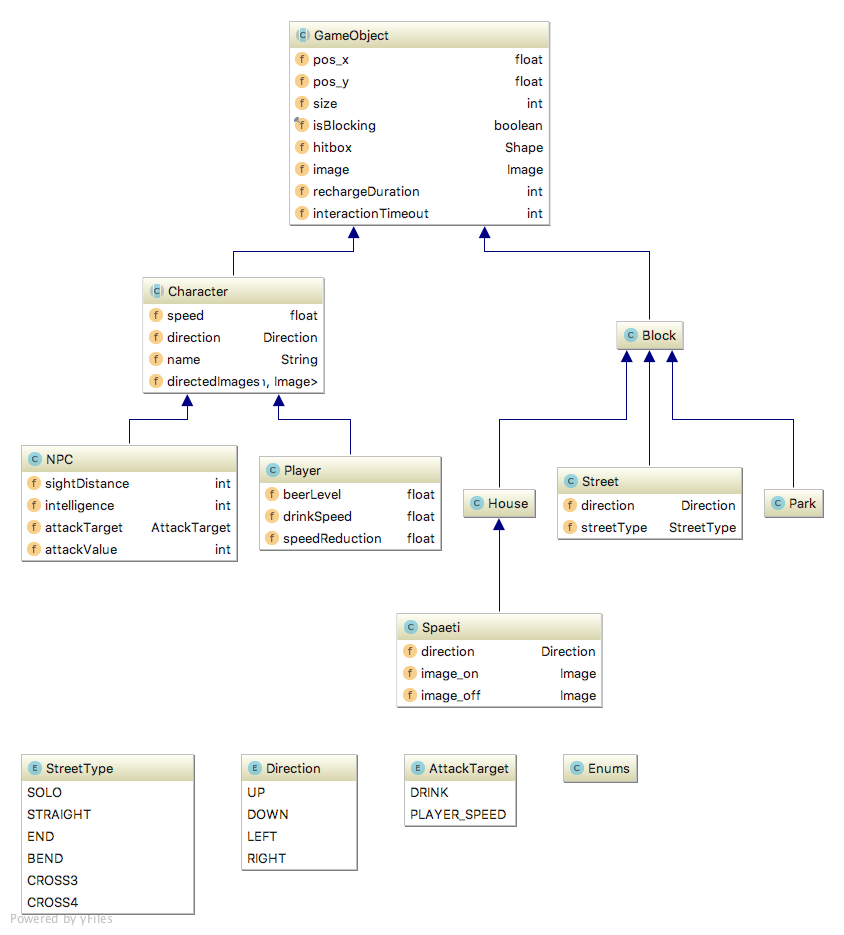
\includegraphics[width=3in]{img/05_model.png}
\caption{Spielobjekte}
\label{fig:spielarchitektur:model}
\end{figure}

\subsection{LevelController}
\label{sub:architektur:levelcontroller}

Der \texttt{LevelController} ist die funktionale Kernkomponente des Spiels.
Zu den wichtigsten Funktionalitäten zählen die Initialisierung eines Levels, die Kollisionskontrolle innerhalb eines Levels sowie die Berechnung der künstlichen Intelligenz der NPCs.
Auf diese Funktionalitäten wird im Folgenden näher eingegangen.

\subsubsection{Initialisierung des Levels}
In der Klasse \texttt{GameObject} in Abbildung \ref{fig:spielarchitektur:model} ist ersichtlich, dass jedes Spielobjekt Informationen über seine eigene Position auf der Spielfläche (\texttt{pos\_x} und \texttt{pos\_y}) besitzt.
Um die Level unabhängig von der Pixelgröße des Ausgabefensters und der Blockgröße zu gestalten, entsprechen diese Positionsangaben zunächst einfachen Indexwerten.
Die Indexwerte entsprechen der Position des entsprechenden Spielobjekts vom oberen linken Spielfeldrand aus.
Es werden zunächst alle Blockindexwerte mit den korrekten pixelbasierten Positionen aktualisiert.
In der aktuellen Implemntierung weisen Blöcke der Karte eine feste Größe von 32x32 Pixeln auf.

Ebenfalls muss Der Typ von \texttt{Street}-Objekten, also ob es sich hierbei beispielsweise um eine Kreuzung oder einer geraden Straße handelt, ermittelt werden.
Dazu wird während der Initialisierung eine Karte der Straßenobjekte in Form eines zweidimensionalen \texttt{boolean[][]}-Arrays erzeugt.
Anhand dieser Karte können nun, für jedes \texttt{Street}-Objekt einzeln, die Nachbarn ermittelt und der korrekte Straßentyp und eine eventuelle Rotation festgestellt werden.

\subsubsection{Kollisionskontrolle}
Der \texttt{LevelController} ermittelt Kollisionen zwischen \texttt{GameObject}-Objekten.
Dazu wird die Methode \texttt{Shape.intersect(Shape)} aus der Slick2D Bibliothek verwendet, welche zwei geometrische Objekte auf eine Schnittmenge untersucht und \texttt{true} zurück liefert sobald eine Schnittmenge existiert.
In diesem Fall berühren sich beide \texttt{GameObject}-Objekte und es wird auf beiden die \texttt{GameObject.interact(GameObject)} Methode aufgerufen.
Dies stellt die Interaktion zwischen zwei \texttt{GameObject} Instanzen sicher.
Innerhalb der konkreten Implementierungen von \texttt{interact()} wird dann unter anderem durch Reflection entschieden, welche Aktionen durchgeführt werden sollen.
In Listing \ref{lst:npc-interact} wird dies anhand der Implementierung der \texttt{interact()} Methode der Klasse \texttt{NPC} deutlich.
Sobald ein Objekt getroffen wird, welches die Eigenschaft \texttt{isBlocking} aufweist, wird eine Zufallsrichtung gewählt.
Wurde der \texttt{Player} getroffen, dann wird er, je nach spezifiziertem Angriffsziel, angegriffen und ein Timeout gesetzt um zu verhindern, dass Angriffe direkt nacheinander erfolgen können.

\begin{lstlisting}[caption={NPC.interact() Implementierung (NPC.java)}\label{lst:npc-interact},captionpos=t,language=Java]
@Override
public void interact(GameObject go) {
 if (go.isBlocking()) {
  this.setDirection(getRandomDirection());
 }
 if (interactionTimeout == 0) {
  if (go.getClass().equals(Player.class)) {
   Player p = (Player) go;
   if (attackTarget == Enums.AttackTarget.DRINK) {
    p.setBeerLevel(p.getBeerLevel() - attackValue);
    this.interactionTimeout = this.rechargeDuration;
   }
   if (attackTarget == Enums.AttackTarget.PLAYER_SPEED) {
    p.attackSpeed(attackValue);
   }
  }
 }
 super.interact(go);
}

\end{lstlisting}

Slick2D ist bestrebt, in regelmäßigen Abständen die implementierte Spiellogik durch Aufruf einer \texttt{update()} Methode zu aktualisieren.
Bei jeder Aktualisierung wird auf Kollisionen geprüft.
Es kann bei zu geringer Aktualisierungsrate, beispielsweise aus Performancegründen, oder zu hoher Geschwindigkeit der bewegenden Spielobjekte dazu kommen, dass einzelne Treffer mit Objekten nicht erkannt, und die Spielobjekte somit über Objekte springen können.
Aus diesem Grund unterteilt der \texttt{LevelController} Bewegungsintentionen in mehrere Teilschritte, prüft diese einzeln und unterbricht die Bewegung sobald eine Kollision innerhalb eines Teilschrittes erkannt wurde.
Dies sorgt auch dafür, dass Spielobjekte sauber an Kanten anderer Spielobjekte stehen bleiben und nicht beispielsweise wenige Pixel davor.


\subsubsection{Künstliche Intelligenz der NPC}
\label{subsub:architektur:ki}
NPC sind in der Lage ihr Umfeld wahrzunehmen und daraus Bewegungsänderungen abzuleiten.
Ihr Wahrnehmungsvermögen wird über zwei Kennzahlen gesteuert - Die Sichtweite und die ``Intelligenz''.
Die Intelligenz ist hierbei eine Wahrscheinlichkeit, mit der auf Wahrgenommenes reagiert wird.
Die \texttt{updateAI()} Methode iteriert über alle vorhandenen NPC und zieht jeweils eine Linie (Sichtlinie) zwischen dem entsprechenden NPC und dem Spieler.
Sofern die Sichtlinie kein optisches Hindernis (Blöcke mit \texttt{isBlocking} Eigenschaft) schneidet, wird geprüft ob die Länge der Sichtlinie im Bereich der Sichtweite des NPC ist.
Sofern dies der Fall ist, wird die beste Richtung zur Bewegung in Richtung des Spielers ermittelt.
Der NPC übernimmt diese Richtung mit der Wahrscheinlichkeit seiner Intelligenz.
\section{Levelerzeugung}\label{sec:levelerzeugung}

In diesem Abschnitt wird das Projekt des Levelgenerators näher erläutert. Die Schwerpunkte liegen dabei auf dem Level Metamodell sowie auf der Codegenerierung aus einer gegebenen Leveldatei. 
 
Dabei wird erklärt, wie eine textuelle Leveldatei aussehen muss. Anschließend wird das Metamodell, das diese DSL beschreibt, verständlich dargestellt.

Abschließend wird in diesem Kapitel der Levelgenerator vorgestellt, mit Augenmerk auf seinen Aufbau und seine Funktionsweise.

\subsection{Aufbau einer NBNO-Datei}
Um ein Level mit dem Levelgenerator zu erzeugen, muss eine textuelle Datei im NBNO Format an den Generator übergeben werden. Eine solche Datei besitzt eine durch die DSL fest vorgegebene Struktur. Diese wird durch die benötigten Levelattribute und Eigenschaften bestimmt.

Zunächst enthält ein Level einen Namen und Levelkonfigurationen (vgl. Listing \ref{lst:nbno-lvlConfig}). Der bisherige Projektstand benötigt als Leveleigenschaft nur die Spielzeit des Levels (entspricht dem rechten Balken des Spiels (vgl. Abb. \ref{fig:einleitung:screenshot})).

Der Spieler selbst erhält Eigenschaften die seine Geschwindigkeit, seine Trinkgeschwindigkeit und das initiale Bierlevel einstellen. Wobei das Bierlevel dem linken Balken entspricht (vgl. Abb. \ref{fig:einleitung:screenshot}) und die Trinkgeschwindigkeit die Geschwindigkeit der Leerung dieses Balkens bestimmt.

\begin{lstlisting}[caption={Level Metadaten und Spieler}\label{lst:nbno-lvlConfig},captionpos=t, language=Java]
levelName: TestName
levelConfiguration {
    levelTime: 40
}
player {
    speed: 50,
    drinkSpeed: 6,
    beerLevel: 30
}
\end{lstlisting}

An diesem Auszug ist der Aufbau einer NBNO-Datei bereits zu erkennen.
Bestimmte Attribute besitzen Eigenschaften die angelehnt an das JSON-Format in geschweiften Klammern aufgelistet werden. Separiert werden diese Eigenschaften durch Kommata.

Dies ist auch im nächsten Auszug gut zu erkennen.
Es werden die Gegnerklassen angelegt und mit bestimmten Eigenschaften ausgestattet (vgl. Listing \ref{lst:nbno-enemies}).
Es wird ein Name an diese Klassen verteilt, durch den zur Laufzeit eine passende Darstellung des Charakters erreicht wird.
Weitere Eigenschaften sind die Geschwindigkeit, das Angriffsziel und die Effektivität des Angriffs (Schaden).
Die künstliche Intelligenz des Gegenspielers wird hier ebenfalls vergeben.
Dabei gibt die erste Zahl seine Sichtweite an und die Zweite die Angabe der Wahrscheinlichkeit einer Richtungsänderung des Charakters. (Die KI wurde in Abschnitt \ref{subsub:architektur:ki} genauer erläutert).

\begin{lstlisting}[caption={Gegnerklassen}\label{lst:nbno-enemies},captionpos=t, language=Java]
enemies {
    1 {
        name: Schnorrer,
        speed: 40,
        attackTarget: DRINK,
        damage: 30,
        ki: (10|30)
    },
    2 {
        name: Polizist,
        speed: 25,
        attackTarget: PLAYER_SPEED,
        damage: 70,
        ki: (24|40)
    }
}
\end{lstlisting}

Wichtig sind auch die Ziffern vor den eigentlichen Gegnereigenschaften. Sie stellen die Repräsentation auf der Map dar, die in der Leveldatei angelegt wird (vgl. Listing \ref{lst:nbno-map}). Der Ausschnitt zeigt einige Zeilen einer Map-Konfiguration. Die Spielkarte wird durch Buchstaben und Ziffern repräsentiert, wobei jedes Zeichen dabei eine eigene Bedeutung hat. Die zuvor erwähnten Ziffern der Gegner stellen hier die Startpositionen eines Gegners der entsprechenden Klasse dar. Auf diese Weise ist es möglich, von einer Klasse mehrere Feinde starten zu lassen.

Das ``X'' ist die Startposition des Spielers. Ein ``H'' steht für ein Haus, ein ``P'' für einen Park und das ``S'' ist das Symbol für eine Straße. Die Spätis werden per Pfeilspitze dargestellt. Je nachdem in welche Richtung die Spitze zeigt, öffnet sich der Späti im Spiel und kann vom Spieler angelaufen werden. In diesem Beispiel bedeutet demnach das ``V'', dass der Späti sich nach unten öffnet.

\begin{lstlisting}[caption={Level Map}\label{lst:nbno-map},captionpos=t, language=Java] 
map {
    H,H,H,H,H,H,H,H,H,H,S,S,S,S,S,S,S,S,S,S,S,S,S,S,S
    P,P,S,S,S,S,S,S,2,H,S,S,S,S,S,S,1,S,S,S,S,S,S,S,S
    P,P,S,S,S,S,S,S,S,H,S,S,S,S,H,H,H,S,S,S,S,S,S,S,S
    H,H,V,H,H,H,S,S,S,H,S,S,S,S,H,H,H,S,S,S,S,S,S,S,S
	[...]
    S,S,S,S,S,S,S,S,S,S,S,X,S,S,S,S,S,S,S,S,S,S,S,S,S
}
\end{lstlisting}

\subsection{Metamodell eines Levels}
Das Metamodell dieses Projekts beschreibt die Struktur und den Aufbau eines Levels des Spiels. Das Modell ist in EBNF verfasst und generiert durch Antlr die Compiler für die gewünschte NBNO-DSL.

Die DSL muss immer gleich aufgebaut sein (vgl. Listing \ref{lst:grammar-structure}). Es muss mit dem Levelnamen begonnen und anschließend die Levelkonfigurationen festgelegt werden. Danach folgt der Spieler und die Gegnerklassen. Abschließend muss ein Spielfeld definiert werden.

Um Wiederholungen zu vermeiden, sind Lexerregeln aufgestellt, die Alphabete und Trenner festgelegen.
Außerdem ist eingestellt, dass alle Leerzeichen und Abstände beim Parsen übersprungen werden.

\begin{lstlisting}[caption={Aufbau und Tokens (LevelGrammar.g4)}\label{lst:grammar-structure},captionpos=t, language=Java] 
file : levelName levelConfigs player enemies map EOF;

// helper definitions
ALPHABET: ('a'..'z' | 'A'..'Z')+;
DIGITS : [0-9]+;
ObjectBeginn:'{';
ObjectEnd: '}';
Separator: ',';
WS : [ \t\n\r]+ -> skip ; // skip witepsaces tabs and linebreaks
\end{lstlisting}
 
Die Definitionen der oben genannten Attribute ähnelt sich sehr, weshalb hier beispielhaft der Ausschnitt der Spielerdefinition erklärt wird. Ein Spieler soll in der DSL als \texttt{player} angeben sein, was hier als Schlüsselwort festgelegt wird (vgl. Listing \ref{lst:grammar-player}). Anschließend folgen die geschweiften Klammern. Die Parserregel legt fest, dass ein Spieler Attribute innerhalb der geschweiften Klammern besitzt. Diese Attribute sind durch Kommata getrennt und beginnen immer mit ihrem Schlüsselwort und einem Doppelpunkt dahinter. 

Der Wert des Attributs ist durch einen Verweis auf eines der möglichen Alphabete angegeben. Durch diese strukturelle Einschränkung werden Listener durch Antlr für jeden Attributwert erstellt. Dadurch ist es möglich beim Parsen im Syntaxbaum direkt an diesem Attribut ``anzuhalten`` und sich den Wert ausgeben zu lassen. Dies erleichtert die semantische Prüfung im Levelgenerator. Die anderen Schlüsselattribute der NBNO-DSL sind nach dem gleichen Schema aufgebaut. 

\begin{lstlisting}[caption={Spielerdefinition (LevelGrammar.g4)}\label{lst:grammar-player},captionpos=t, language=Java] 
//the player and its attributes
player: 'player' ObjectBeginn playerAttributes ObjectEnd ;
playerAttributes:  speed Separator drinkSpeed Separator beerLevel;
speed: 'speed:' speedValue;
speedValue: DIGITS;
drinkSpeed: 'drinkSpeed:' drinkSpeedValue;
drinkSpeedValue: DIGITS;
beerLevel: 'beerLevel:' beerLevelValue;
beerLevelValue: DIGITS;
\end{lstlisting}

\subsection{Levelgenerator}

Als Modellinterpretierer und damit Levelgenerator fungiert eine Java Klasse \texttt{LevelGenerator.java}. In ihr werden die durch Antlr erzeugten Lexer und Parser ausgeführt, eine semantische Prüfung der übergebenen Daten vollzogen und abschließend eine Java Leveldatei erzeugt. Diese Levelklasse beerbt das in Abschnitt \ref{sub:architektur:level} beschriebene \texttt{AbstractLevel}. Auf diese Weise kann ein erzeugtes Level einfach mittels Reflection im NBNO-Projekt eingebunden werden, ohne das Änderungen im Quellcode des Spiels von Nöten sind.

Ein sehr wichtiger Bestandteil des Generators ist das \mbox{Errorhandling}. Die Antlr Parser und Lexer werfen standardisiert keine Fehler sondern geben lediglich auf der Konsole eine Nachricht aus, das ein Fehler beim Parsen aufgetreten ist. Gewünscht ist jedoch, dass der Levelgenerator die Erzeugung, bei jeglicher Art eines Fehlers, mit einer Java-Exception abbricht. Aus diesem Grund wird der Antlr \texttt{BaseErrorListener} beerbt und der eigene \texttt{LevelErrorListener} dem Parser und Lexer im Levelgenerator übergeben. Er überschreibt, die bei einem Syntaxfehler aufgerufene Methode und kann so eine Exception werfen, die den Levelerzeugungsvorgang abbricht.

Der Generator liest zu Beginn eine NBNO-Datei aus dem \texttt{levelfiles} Projektverzeichnis ein, deren Dateiname über die Konsole übergeben wird. Dieses File wird dann geparst und auf fehlerhafte Einträge oder Strukturen geprüft. Entspricht die Datei der Grammatik, wird eine Javaklasse mit dem in der Leveldatei spezifizierten Namen angelegt und gespeichert.

Durch das Metamodell ist die syntaktische Analyse bereits abgedeckt, weshalb im Generator die semantische Prüfung fokussiert wird. Dafür werden die erzeugten Listener-Methoden für die Attribute und Attributwerte überschrieben. Im folgenden Codeauszug (vgl. Listing \ref{lst:codegen-lvlName}) wird der Levelname auf Länge (maximal 100 Zeichen) geprüft. Des weiteren wird bei Korrektheit das erste Zeichen zu einem Großbuchstaben gewandelt, so dass die Javaklasse den Javakonventionen entspricht. Ist der Levelname zu lang, so wird ein Fehler geworfen und der Generierungsvorgang abgebrochen.

\begin{lstlisting}[caption={Levelnamensprüfung (LevelGenerator.java)}\label{lst:codegen-lvlName},captionpos=t,language=Java, firstnumber=105]
@Override
public void enterLevelNameValue(LevelGrammarParser.LevelNameValueContext ctx) {
  final String name = ctx.getText();
  if(name.length() > 100){
    throw new IllegalArgumentException(
      GeneratorUtils.getFormattedErrorMessage("Level name is to long!", ctx.getStart()));
  }
  levelName = name.substring(0,1).toUpperCase() + name.substring(1);
}
\end{lstlisting}

Die weiteren Attribute und Eigenschaften werden auf die gleiche Art und Weise geprüft. Beispielsweise wird die Geschwindigkeit des Spielers auf einen Wertebereich zwischen 0 und 100 in der überschriebenen Methode \texttt{enterSpeedValue()} geprüft. So ist gewährleistet das am Ende alle Attribute auch die inhaltlich korrekten Werte enthalten. 

Eine weitere interessante Prüfung geschieht bei der Spielkartenanalyse (vgl. Listing \ref{lst:codegen-mapCheck}). Die Map muss immer genau 20 Zeilen und 25 Spalten enthalten. Wobei Spalten in diesem Projekt als Blöcke interpretiert werden. Ein Block wird im Spiel zu einem 32x32 Pixel Block umgerechnet. Auf diese Weise besitzt das Spielfeld immer die gleiche Größe. Die Leveldateien müssten so auch nicht bearbeitet werden, falls die Größen im Spiel einmal skaliert werden sollten.

\begin{lstlisting}[caption={Map Prüfung (LevelGenerator.java)}\label{lst:codegen-mapCheck},captionpos=t,language=Java, firstnumber=230]
@Override
public void enterMapValue(LevelGrammarParser.MapValueContext ctx) {
  final int maxRows = 20;
  final int maxBlocks= 25;
  if(ctx.row().size() != maxRows){
      throw new IllegalArgumentException("The map must have 20 rows. Not more or less.");
  }
  int rowCounter = 0;
  int blockCounter = 0;
  for(LevelGrammarParser.RowContext row : ctx.row()){
      if(row.block().size() != maxBlocks){
          throw new IllegalArgumentException("Each row in the map must contain " + maxBlocks + " Blocks. "
                  + "In Line " + row.getStart().getLine() + "is an incorrect number of blocks.");
      }
      for(LevelGrammarParser.BlockContext block : row.block()){
          final int xPos = blockCounter;
          final int yPos = rowCounter;
          final String blockVal = block.getText();
          switch (blockVal){
            case GeneratorUtils.HOUSE:
               generateHouseString(xPos, yPos);
               break;
            [...]
            default:        // wenn keins der oberen matched, muss es eine Zahl sein
               generateEnemyString(Integer.parseInt(blockVal), xPos, yPos);
               generateStreetString(xPos, yPos);
               break;
          }
          blockCounter ++;
      }
      blockCounter = 0;
      rowCounter ++;
  }
}
\end{lstlisting}

Ein weiteres Detail wird in dieser Methode ebenfalls sichtbar. Beim Durchlaufen der einzelnen Blöcke der Karte wird für jeden Block ein String angelegt. Diese Strings werden in einer Liste von Strings gesammelt.

Alle variablen Attribute, wie der Spieler oder die Gegnerklassen,  werden als Strings erzeugt. Zu beachten ist, dass unter jedem Gegner und dem Spieler jeweils noch ein Straßenblock erzeugt werden muss. All diese erstellten Zeichenketten werden in Listen gespeichert. 

Die Codegenerierung erfolgt am Ende durch das Zusammensetzen aller gespeicherten Strings. Alle Konstanten Angaben, wie der Import von Datentypen oder das Überschreiben des Konstruktors, werden zuvor in der Methode \texttt{generateLevelClass()} mit den anderen variablen Strings in einer Liste zusammengeführt. Diese enthält dann die komplette Levelklasse als Stringrepräsentation.
 
Über die final entstandene Stringliste wird in der \texttt{writeFile()} Methode iteriert und für jeden String eine eigene Zeile in die neue Javaklasse geschrieben.

Ist ein Level erfolgreich erstellt, muss diese Javadatei in das \texttt{level} Package des Spielprojekts kopiert werden. Wird das Spiel dann gestartet steht das Level zur Verfügung. Dies ist das Bindeglied zwischen den zwei Projekten.\todo{evtl. rausnehmen den bindegleidsatz}

\section{Fazit}

Das Ziel dieses Software-Engineering Projekts war es, durch einen ansprechenden Rahmen, Codegenerierung anzuwenden und besser kennenzulernen.
In diesem Projekt wurde die Codegenerierung bei der Levelgenerierung für ein selbstgeschriebenes 2D Spiel namens NBNO angewendet.

Das Spiel hält einen Spieler dazu an, stetig sein Bier aufzufüllen und dabei schadenden Gegnern auszuweichen.
Das Spielprinzip und die Umsetzung sind sehr gelungen und ein Spaßfaktor ist dem Spiel nicht abzusprechen.

Die Level dieses Spiels werden im Levelgenerator erzeugt, der aus einer textbasierten NBNO-Datei eine Javaklasse generiert, die in das Spiel eingebunden werden kann.

Beide Projektteile sind gelungen und harmonieren in gemeinsamer Verwendung. Demnach ist das Projektziel durch die Umsetzung erreicht worden.

Die verwendeten Technologien Slick2D und Antlr waren für die Umsetzung sehr nützlich und hilfreich.
Die Arbeitsweise mit diesen Werkzeugen ist als effizient und zielfördernd anzusehen, weshalb bei ähnlichen Problemstellungen einer Wiederverwendung dieser Tools zu empfehlen ist.
\section{Ausblick}

- mehr verschiedene Blöcke
- dynamische Spielfeldgröße (bei anpassbarem Fenster mit Scrolling)
- Was hätte man mit mehr Zeit noch machen können?
- Scaling auf Fullscreen, alles zu abhängig von Pixeln
- Level Schwieirgkeiten und Level freischalten
- weitere gegner klassen, parkbänke etc.
- Konfiguration der späti ladezeit in dsl


% conference papers do not normally have an appendix



% trigger a \newpage just before the given reference
% number - used to balance the columns on the last page
% adjust value as needed - may need to be readjusted if
% the document is modified later
%\IEEEtriggeratref{8}
% The "triggered" command can be changed if desired:
%\IEEEtriggercmd{\enlargethispage{-5in}}

% references section

% can use a bibliography generated by BibTeX as a .bbl file
% BibTeX documentation can be easily obtained at:
% http://www.ctan.org/tex-archive/biblio/bibtex/contrib/doc/
% The IEEEtran BibTeX style support page is at:
% http://www.michaelshell.org/tex/ieeetran/bibtex/
%\bibliographystyle{IEEEtran}
% argument is your BibTeX string definitions and bibliography database(s)
%\bibliography{IEEEabrv,../bib/paper}
%
% <OR> manually copy in the resultant .bbl file
% set second argument of \begin to the number of references
% (used to reserve space for the reference number labels box)
\begin{thebibliography}{1}

\bibitem{IEEEhowto:kopka}
H.~Kopka and P.~W. Daly, \emph{A Guide to \LaTeX}, 3rd~ed.\hskip 1em plus
  0.5em minus 0.4em\relax Harlow, England: Addison-Wesley, 1999.

\end{thebibliography}




% that's all folks
\end{document}


